% Harmonic potential and symmetric turning points. Reference: handdraw/harmonic.png.
% Compile: pdflatex harmonic_tikz.tex
\documentclass[tikz,border=6pt]{standalone}
\usepackage{amsmath}
\usepackage{fix-cm}
\usetikzlibrary{arrows.meta}
\begin{document}
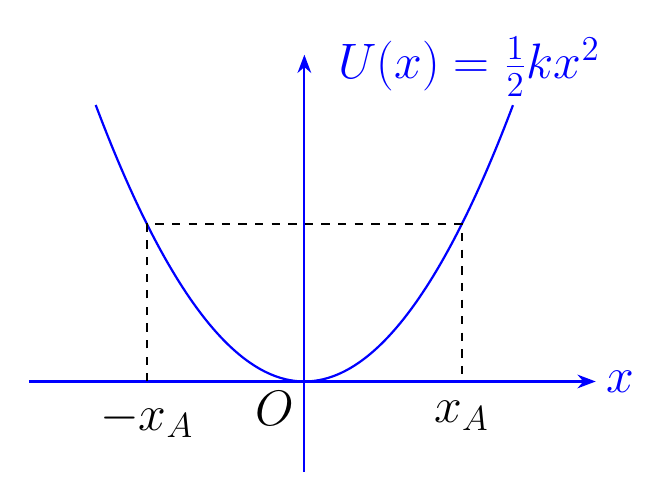
\begin{tikzpicture}[>=Stealth,thick,every node/.style={font=\fontsize{18}{22}\selectfont}]
  \draw[blue,->] (-3.5,0) -- (3.7,0) node[right] {$x$};
  \draw[blue,->] (0,-1.15) -- (0,4.15);
  \node[blue,anchor=west] at (.3,4.0) {$U(x)=\frac12 kx^2$};
  \draw[blue,domain=-2.65:2.65,samples=100,smooth] plot (\x,{.5*\x*\x});
  \draw[dashed] (-2,0) -- (-2,2) -- (2,2) -- (2,0);
  \node[below] at (-2,-.12) {$-x_A$};
  \node[below] at (2,-.12) {$x_A$};
  \node[below left] at (0,0) {$O$};
\end{tikzpicture}
\end{document}
